\documentclass[natbib]{article}
\usepackage{microtype}
\usepackage{lmodern}
\usepackage{url}
\usepackage{xspace}
\usepackage{calc}
\usepackage{enumerate}
\usepackage{listings}
\usepackage{amsmath,amssymb}
\usepackage{rotating}
\usepackage{colortbl}
\usepackage{pifont}
\usepackage{tikz}
%\usetikzlibrary{shapes,shadows,arrows,calc,positioning,fit,matrix,mindmap,trees}
%\usepackage{pgfplots}
%\usepackage{pgfplotstable}
\usepackage{booktabs}
\usepackage{natbib}
\usepackage{colortbl}
\usepackage{algorithm2e}
\usepackage{syntax}
% pantone colors

% More sensible defaults akin to \sloppy
% \tolerance 1414
% \hbadness 1414
% \emergencystretch 1.5em
% \hfuzz 0.3pt
% \widowpenalty=10000
% \clubpenalty=10000
% \vfuzz
% \hfuzz
% \raggedbottom

\newcommand{\ignore}[1]{}
\newcommand{\st}{\textit{s.\,t.}\xspace}
\newcommand{\eg}{\textit{e.\,g.}\xspace}
\newcommand{\ie}{\textit{i.\,e.}\xspace}
\newcommand{\cf}{\textit{cf.}\xspace}

\newcommand{\blackarrow}{{\color{black} \Pisymbol{pzd}{217}}}
\newcommand{\redarrow}{{\color{DarkRed} \Pisymbol{pzd}{217}}}
\newcommand{\minibox}[2]{\begin{minipage}{#1}\raggedright #2\end{minipage}}

\newcommand{\enquote}[1]{``#1''}

%\newcommand{\fixme}[1]{\begin{tikzpicture}
%\node[bottom color=red!80!white, top color=red!70!black, rounded corners,
%      font=\bf\color{white}\footnotesize] {
%  \begin{minipage}{.75\columnwidth}
%    FIXME\\
%    #1
%  \end{minipage}
%};
%\end{tikzpicture}
%}

\lstset{
  language=C,
  basicstyle=\small,%\scriptsize, %\footnotesize\ttfamily,
  keywordstyle={\bf},
  keywordstyle={[2]\it},%\color{Blue!40!black}},
  breaklines=true,
  identifierstyle=,
  stringstyle=\bf,
  commentstyle=\it\color{black!80},
  captionpos=b,
  numbers=left,
  stepnumber=3,
  columns=fullflexible
}

\begin{document}
\title{Typeforge User Manual\\Version 0.6.0}

\author{\small Markus Schordan, Nathan Pinnow}
%\end{tabular}
\date{January 11, 2019}

\maketitle

%\begin{abstract}
%\noindent Typeforge is a tool for analysis and transformation of variable types in 
%C/C++ programs. The main focus of development was to aid the development of 
%mixed-precision programs through modification and searching of the AST. 
%Typeforge does this through changing type information and inserting program 
%instrumentation then outputting modified source code for the user or other tools to use.
%
%\end{abstract}

\tableofcontents

%-------------------------------------------------------------------------

\section{Introduction}
\label{sec:intro}

Typeforge is based on the ROSE compiler infrastructure\footnote{\url{http://www.rosecompiler.org/}} 
and uses the ROSE abstract syntax tree as basis for its transformations. 
A main focus of Typeforge development was as part of a tool pipeline designed for 
the automatic generation of mixed-precision programs. For use in the pipeline 
Typeforge works with ADAPT~\cite{adapt} to insert the needed instrumentation to 
perform automatic differentiation for the purpose of finding variables error threshold.
Typeforge was also designed to work with CRAFT~\cite{CRAFT2013PARCO,CRAFT2013ICS,CRAFT2016} 
for the purpose of searching mixed-precision configurations built by Typeforge 
for the best performance.

\subsection{CRAFT-ADAPT Pipeline}\label{sec:pipeline}
\begin{figure}[h]
    \centering
    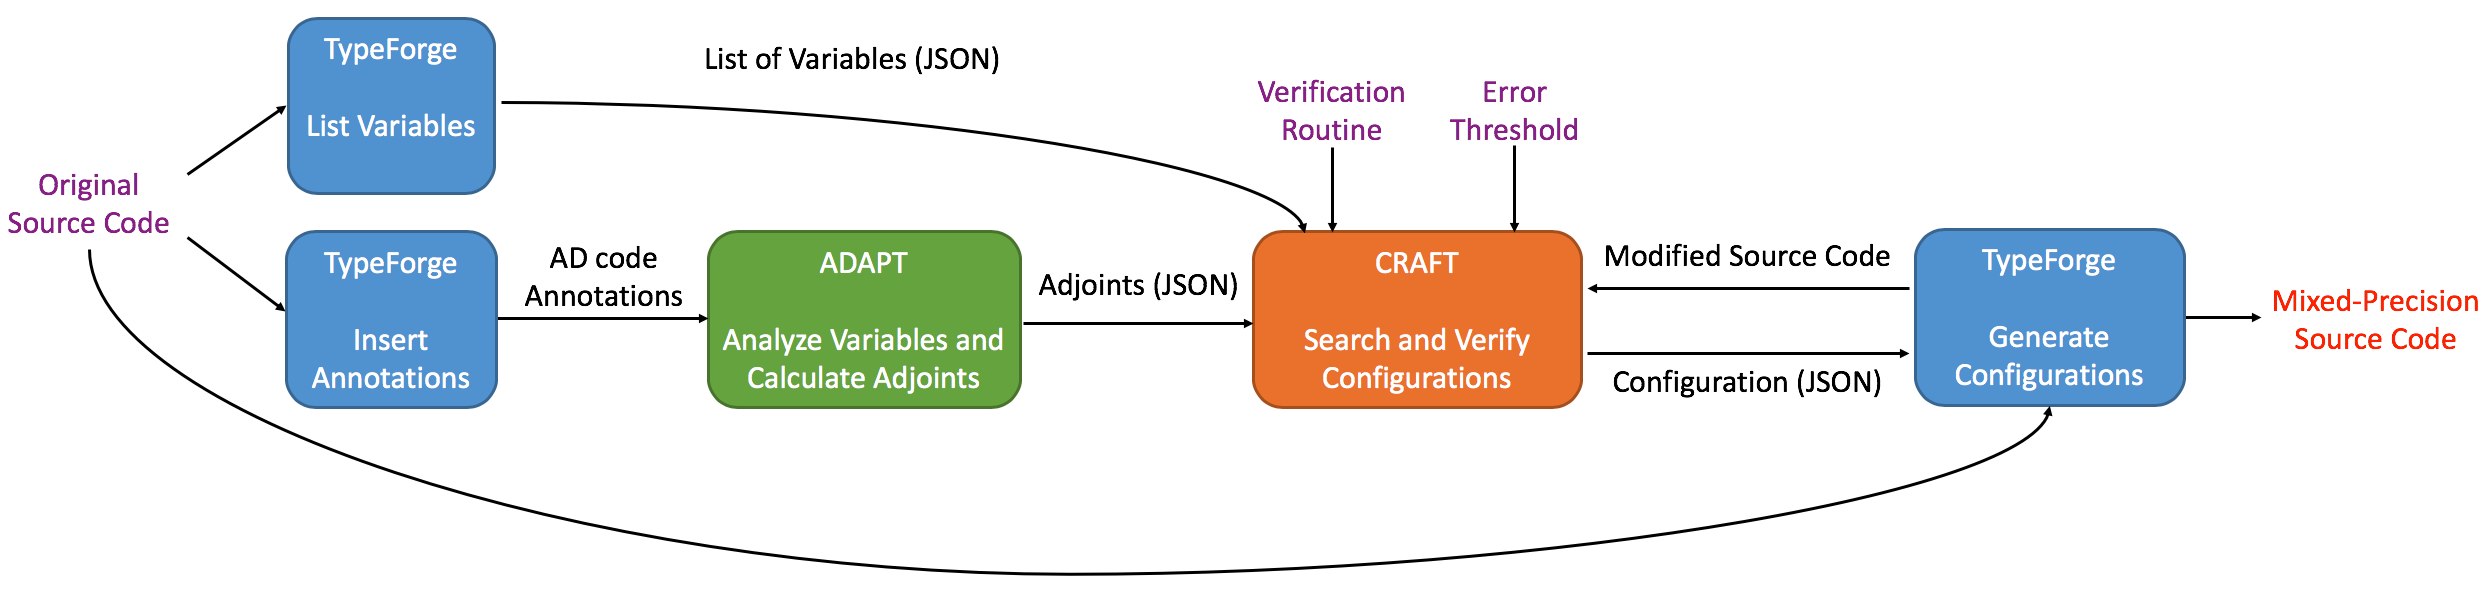
\includegraphics[width=\textwidth]{pipeline.png}
    \caption{\textsf{Diagram of pipeline structure}}
    \label{fig:pipeline}
\end{figure}
\noindent
Typeforge has several uses in the pipeline for automatic generation of mixed precision programs
as seen in figure \ref{fig:pipeline}. 
In order for craft to conduct a proper search it needs to define 
a search space which can be done by Typeforge by looking for all declarations in the AST. This 
list can be refined by looking at sets to avoid searching configurations that will not compile. 
When CRAFT tests a configuration it passes the appropriate plugin to Typeforge so 
that it can generate new source code and compile the configuration. This lets CRAFT gain 
performance metrics on a configuration instead of estimations. To refine the search space ADAPT 
feeds precision information to CRAFT but for ADAPT to run modifications need to be made to the 
source code. These modifications are pragma replacement, adding includes, replacing floating point 
types with AD\_real, and adding ADAPT function calls. All of the ADAPT modifications and Variable 
listing can be done with Typeforge with a single plugin shown in section \ref{sec:expampleSpec}.

\section{Installation}

First step is to install ROSE which will also configure Typeforge but not install
by default as part of ROSE. to install Typeforge after installing ROSE run
'make install' and optionally 'make check' in the \verb+projects/+ \verb+typeforge+ directory to 
install Typeforge. Typeforge is installed as 'typeforge' (at the same location as other ROSE tools, 
in the 'bin' directory of the ROSE installation).

\section{Command Line Options}
The command line options of Typeforge are parsed by Boost's program options 
library\footnote{\url{http://www.boost.org/doc/libs/1_63_0/doc/html/program_options.html}}.
The following command line options are listed when running \verb+typeforge --help+.
These main options below comprise general parameters such as spec file and explicit command line 
transformation. All filenames and unrecognized options will be passed directly to the ROSE compiler 
as command line options.

\begin{verbatim}
typeforge <filename> [OPTIONS]
Supported Options:
  -h [ --help ]                   Produce this help message.
  
  -v [ --version ]                Display the version of Typeforge.
  
  --compile                       Run backend compiler.
  
  --explicit                      Make all implicit casts explicit. This option can be
                                  used to make all implicit cases visible to the user in
                                  the (genrated) program source.
  
  --cast-stats                    Print statistics on casts of built-in 
                                  floating point types.
                                  
  --stats                         Print statistics on changes performed on the
                                  input program.

  --trace                         Print program transformation operations 
                                  as they are performed.

  --plugin arg                    Name of Typeforge plugin files.
  
  --csv-stats-file arg            Generate file [args] with transformation statistics.
  
  --typeforge-out                 File to store output inside of JSON.
  
\end{verbatim}
\section{Plugin Definition File}
To define what actions Typeforge should perform it uses a JSON file as a format for the plugin definition. The JSON file is generated using ToolConfig and was designed to allow for other programs to create specifications for Typeforge. The ToolConfig JSON has several header string fields named executable, tool\_id, version, and a list of strings named source\_files. These fields are not used for input to Typeforge and a designed for information tracking. For providing the actions to Typeforge ToolConfig has a list of ToolAction named actions. Each item in the actions list is also a JSON object with each item defining an action for Typeforge to take. All actions have an analysis phase and some will have an execution phase where they will make modifications to the AST. The separation of phases allows for an action to find a change and later make the change without another action finding a change location based upon the changed code. If actions contradict the behavior is undefined.

\subsection{Handles} \label{sec:handles}
Several actions are related to the use of compiler generated handles. Typeforge is capable of emitting string 
based handles for the purpose of variable and function identification. These handles are guaranteed to 
uniquely identify a variable or function in the program and can be used to specify them to Typeforge. 
The content and format of these handles is not guaranteed and is 
subject to change.

\subsection{Actions}
The grammar below defines how the plugin definition file is made.
The symbols "$\langle\rangle$" are used to indicate a non-terminal, the symbol "$\mid$" is used to 
indicate alternative, "()*" is used to indicate repeat what is in the group zero or more times. 
All other symbols are terminal. 

\begin{grammar}
<PluginDefinitionFile> ::= \{''actions'' : [<Action>(, <Action>)*]\}

<Action>                 ::= <ActionID>, ((<Scope>, <Name>) | <Handle>), <ToType>
\alt <ActionID>, <Scope>, <FromType>, <ToType>
\alt <ActionID>, <Scope>, <Name>
\alt <ActionID>, <Scope>,
\alt <ActionID>, <FromType>, <ToType>

<ActionID> ::= ''"action"'': ''<ActionSpecifier>''

<Scope> ::= ''"scope"'': ''<ScopeSpecifier>''

<Name> ::= ''"name"'': ''<NameSpecifier>''

<ToType> ::= ''"to_type"'': ''NewType''

<FromType> ::= ''"from_type"'': ''MatchType''

<Handle> ::= ''"handle"''":" ''CompilerHandle''
\end{grammar}

\subsubsection{Var Type Change} \label{sec:vartypechange}
This action is for changing the type or base type of a specified variable. Actions related to 
changing type end in type or basetype which is used to specify how the change should be made. 
When type is used the type will be changed and potentially matched based on the exact type 
regardless of pointers and arrays. When basetype is used Typeforge will match and change types 
by stripping away then rebuilding arrays, pointers, typedefs, reference, and modifiers. 
Scope can be either the name of the function where the variable is located or "\$global" 
for a global variable. Name can be the name of a single variable or a comma separated 
list of variables to change. A handle can be specified instead of using scope and variable name. New type 
should be the type that the variable will be changed to.

\begin{grammar}
<ActionSpecifier> ::= "change_var_type" | "change_var_basetype"

<ScopeSpecifier>    ::= FunctionName | "\$global"

<NameSpecifier>     ::= VariableName(,VariableName)*
\end{grammar}
\begin{verbatim}

Example:
{
  "action": "change_var_basetype",
  "scope": "main",
  "name": "x",
  "to_type": "float"
},
{
  "action": "change_var_basetype",
  "handle": "Project<numbering,1>::FileList<numbering,1>::SourceFile
              <name,/home/src/main.C>::VariableDeclaration<position,7.1-7.15>",
  "to_type": "float"
}
\end{verbatim}

\subsubsection{Change Type} \label{sec:chagetype}
This action is to replace all variables of a type with a new type. Match\_Type is the type that Typeforge
will search for and New\_Type is the type that it will replace match type with.
Scope is the locations where variables should be changed and has several forms. 
Use "\$global" to specify replacing globals, otherwise use function name followed by colon 
then parts of the function to change in a comma separated list. Use args to change arguments, 
body to change the body of the function, and ret to change the return type. The function name 
can be replaced with * to change all functions. For example to change everything in main use 
"main:args,ret,body". See section \ref{sec:vartypechange} for more information on type changing. 

\begin{grammar}
<ActionSpecifier>  ::= "change_every_type" | "change_every_basetype"

<ScopeSpecifier>     ::=  FunctionName:<VariableLocationList> 
\alt "*":<VariableLocationList> | "\$global"

<VariableLocationList> ::= <VariableLocation>(, <VariableLocation>)*

<VariableLocation> ::= "args" | "ret" | "body"

\end{grammar}
\begin{verbatim}

Example:
{
  "action": "change_every_type",
  "scope": "*:body",
  "from_type": "double",
  "to_type": "AD_real"
}
\end{verbatim}

\subsubsection{Listing Changes} \label{sec:listChange}
Will output a list of possible replacements that have the same type as Match\_Type without changing the type. 
Will output a JSON file with the actions set so when input as a plugin will result in the changes being made. 
The output list will include the scope name and compiler handle. Scope is a function name, * for all functions, 
or \$global for global variables. Scope can also be omitted for Typeforge to examine the entire program. 
New\_Type is only used for writing a valid plugin definition file to output. 
See section \ref{sec:vartypechange} for more information on type changing. 

\begin{grammar}
<ActionSpecifier>  ::= "list_changes_type" | "list_changes_basetype"

<ScopeSpecifier> ::= FunctionName | "*" | "\$global"
\end{grammar}
\begin{verbatim}  

Example:
{
  "action": "list_changes_basetype",
  "scope": "",
  "from_type": "double",
  "to_type": "float",
}
\end{verbatim}

\subsubsection{ADAPT Instrumentation}
Inserts ADAPT function calls where appropriate. Will look for any location in the AST where a floating 
point type is assigned to or initialized then insert the correct AD\_intermidiate function 
call after the assignment with the name passed to ADAPT being set to the variables handle. 
If "\#pragma adapt begin" is included in the body will insert instrumentation for initialized 
globals immediately after the pragma. Will not do type replacement for AD\_real, including 
of ADAPT headers, or adapt pragma replacement. Scope is the function name where 
instrumentation should be inserted or "*" for all functions.

\begin{grammar}
<ActionSpecifier> ::= "ad_intermediate_instrumentation"

<ScopeSpecifier>     ::=  FunctionName | "*"
\end{grammar}
\begin{verbatim}  

Example:
{
  "action": "ad_intermediate_instrumentation",
  "scope": "*"
}
\end{verbatim}

\subsubsection{Add Include}
Will add include to files in the AST. Scope is used to specify  to
only insert the include in files that define a specific function or use "*" for all files. 
Name is the name of the file to be included.

\begin{grammar}
<ActionSpecifier> ::= "add_include"

<ScopeSpecifier>     ::=  FunctionName | "*"

<NameSpecifier>     ::= FileName
\end{grammar}
\begin{verbatim}

Example:
{
  "action": "add_include",
  "scope": "main",
  "name": "adapt-impl.cpp"
}
\end{verbatim}

\subsubsection{Pragma Replacement} 
Will perform simple pragma replacement inside the AST. Will only 
replace pragmas that begin with MatchType excluding the \#pragma. NewType is what the 
pragma will be replaced with. Can specify arguments by writing \$N where N is the argument 
number with 0 being the first token after the pragma in the source file including the matched string.

\begin{grammar}
<ActionSpecifier>  ::= "replace_pragma"
\end{grammar}
\begin{verbatim}

Example:
{
  "action": "replace_pragma",
  "from_type": "adapt begin",
  "to_type": "AD_Begin();"
}
\end{verbatim}

\subsection{Example Spec Files} \label{sec:expampleSpec}
\subsubsection{Pipeline Initial Start}
This plugin definition file is used as setup for the pipeline in section \ref{sec:pipeline}. 
Note there is an action to change all doubles to AD\_real and an action to 
list replacements for doubles. These can both work as they are performed on the original tree.
\begin{verbatim}
{
  "version": "1",
  "tool_id": "Master",
  "actions": [
    {
      "action": "replace_pragma",
      "from_type": "adapt begin",
      "to_type": "AD_begin();"
    },
    {
      "action": "add_include",
      "name": "adapt-impl.cpp",
      "scope": "main"
    },
    {
      "action": "transform",
      "scope": "*",
      "from_type": "float",
      "name": "ad_intermediate_instrumentation"
    },
    {
      "action": "change_every_basetype",
      "scope": "*:args,ret,body",
      "from_type": "double",
      "to_type": "AD_real"
    },
    {
      "action": "list_changes_basetype",
      "scope": "",
      "from_type": "double",
      "to_type": "float",
      "name": "outputFile.json"
    }
  ]
}
\end{verbatim}

\subsubsection{CRAFT Configuration}
This plugin file is to change the type of two specific variables to float types.
One change is based upon the handle while the other is based upon specifying function 
name and variable name.

\begin{verbatim}
{
  "version": "1",
  "tool_id": "CRAFT",
  "actions": [
  	{
  	  "action": "change_var_basetype",
  	  "handle": "Project<numbering,1>::FileList<numbering,1>::SourceFile
                  <name,/home/src/test.C>::VariableDeclaration<position,1.1-1.15>",
      "to_type": "float"
    }
    {
  	  "action": "change_var_basetype",
      "scope": "main",
      "to_type": "float",
      "name": "x"
    }
  ]
}
\end{verbatim}

\section{Experimental Features} \label{analysis}
\subsection{Variable Sets}
When changing the type of a variable it is possible that changing types will result in a 
compilation error due to interdependent variables. This happens when variables are connected, 
such as through assignment, and the types cannot simply be cast to be the same as with pointers 
or arrays. This results in every variable being part of a dependence set where all the variables 
in a given set must be changed together or the program will fail to compile. Given how these 
dependence sets are defined all variables will be part of a class and the classes will not intersect. 
Section \ref{sec:setAlg} shows the algorithm for set generation for just variables and 
section \ref{sec:setDef} shows a definition for the sets.
\subsubsection{Sets Definition} \label{sec:setDef}
Let V be a set of all variables, function parameters, and function return types.
Let M be a set of variable sets showing what a variable is directly related to. Each Variable is associated with a single set.
Let S be resulting fully connected sets with the following properties.

\begin{gather*} 
\forall i \in V(\exists! j \in S(i \in j))\\
\forall x \in M(\exists! y \in S(x \cap y \neq \emptyset) \wedge 
\exists! z \in S(x \subseteq z))
\end{gather*}

\subsubsection{Sets Algorithm} \label{sec:setAlg}
\begin{algorithm}[H]
\label{variableSetAlgo}
\SetAlgoLined
\KwResult{Dependence\_Sets}
Map$\langle$Node,Set$\langle$Node$\rangle\rangle$ Dependence\_Map;\\
List$\langle$Set$\langle$Node$\rangle\rangle$ Dependence\_Sets;\\
\For{Variable $\in$ All\_Variables}{
  Dependence\_Map.Add(Variable, Variable);
}
 \For{Node $\in$ All AST Nodes}{
   \If{Node == Expression and Node.type == [Pointer or Array]}{
     \If{Node == Assignment\_Node}{
       Destination  = Left  Hand Side;\\
       Origin       = Right Hand Side;\\
       \For{VarRef $\in$ All Variable References in Origin}{
       Dependence\_Map.Add(VarRef, Destination);\\
       Dependence\_Map.Add(Destination, VarRef);
       }
     }
   }
 }
 \For{Variable\_Set $\in$ Dependence\_Map}{
   Matched = Null;\\
   \For{Set $\in$ Dependence\_Sets}{
     \If{Variable\_Set Intersects Set}{
       \eIf{Matched}{
         Matched.add(Set);\\
         Dependence\_Set.Remove(Set)
       }{
         Set.add(Variable\_Set);\\
         Matched = Set;
       }
     }
   }
   \If{Not Matched}{
     Dependence\_Sets.Add(Variable\_Set)
   }
 }
 \caption{Algorithm for building variable sets}
\end{algorithm}

\subsubsection{Set List Action}
This action functions the same as listing changes in section \ref{sec:listChange}. The difference is instead 
of listing every action as a separate change the connected variables will be part of a single action 
separated by '=='. When sent back to Typeforge as a plugin it will change the variables as an atomic action.

\begin{grammar}
<ActionSpecifier>  ::= "'set_changes_basetype'"
\end{grammar}
\begin{verbatim}  

Example:
{
  "action": "set_changes_basetype",
  "from_type": "double",
  "to_type": "float",
}
\end{verbatim}

\subsubsection{Change Variable Set Action}
This command is similar to the change variable type action in section \ref{sec:vartypechange}. 
The difference with this command is once it finds the variable to change it will look up the set for 
that variable and change the entire set as an atomic action based on a representative element.

\begin{grammar}
<ActionSpecifier> ::= change_set_basetype
\end{grammar}
\begin{verbatim}

Example:
{
  "action": "change_set_basetype",
  "scope": "main",
  "name": "x",
  "to_type": "float"
}
\end{verbatim}

\bibliographystyle{plain}
\bibliography{typeforge}

\end{document}

